% Drawing 148/04-1 -- folder 148, batch 04, archive page 66 (PDF page 67).
% Transcription: Dessins de la page. À gauche, à l'encre rouge et noire, la sphère à trois trous $0$, $1$, $\infty$ subdivisée : sur le bord du trou $0$ les points $a^0_1, \ldots, a^0_4$ et $b^0_1, \ldots, b^0_5$, sur le trou $1$ les points $a^1_1, a^1_2, a^1_3$ et $b^1_1, \ldots, b^1_4$, sur le cercle extérieur $\infty$ les points $a^\infty_1, a^\infty_2, a^\infty_3$ et $b^\infty_1, \ldots, b^\infty_5$, reliés deux à deux par des arcs. En dessous, des cercles orientés, dont l'un marqué « $[0, \alpha][1, \beta)$ » (lecture douteuse), et deux triangles de sommets $0$, $1$, $\infty$ : le premier avec $\alpha = 3$ (points $a_1, a_2, a_3$ sur le côté $1\infty$), $\beta = 5$ ($b_1, \ldots, b_5$ sur $0\infty$), $\gamma = 4$ ($c_1, \ldots, c_4$ sur $01$) ; le second avec la suite « $c_1 c_2 c_3 c_4 \cdot b_5 b_4 b_3 b_2 b_1$ ». Au centre, un petit triangle subdivisé ($b_1, \ldots, b_5$, $a_1, a_2, a_3$, $c_1, \ldots, c_4$) ; à droite, une carte trivalente et les régions $A_{0\infty}$, $A_{01}$, $A_{10}$, $A_{1\infty}$, $A_{\infty 0}$, $A_{\infty 1}$ au crayon
% Kind: page of drawings: subdivided pair of pants, oriented circles, subdivided triangles, trivalent map. Method 2 (schematic redraw from the facsimile). Status: partial.
% Notes: Whole half-page. Left: the sphere with three holes 0, 1, infinity (outer circle), with the points a^0_1..a^0_4, b^0_1..b^0_5 on hole 0, a^1_1..a^1_3, b^1_1.. on hole 1, a^inf_1..a^inf_3, b^inf_1..b^inf_5 on the outer circle, and the arcs joining them (approximate; the hole boundaries drawn red after the transcription, colour faint on the render). Below: oriented circles, one marked [0, alpha][1, beta) (doubtful reading kept), two triangles 0, 1, infinity (alpha = 3, beta = 5, gamma = 4 with a_i, b_i, c_i; the second with c_1c_2c_3c_4 . b_5...b_1), a small subdivided triangle in the centre. Right: a trivalent map (schematised) and the region labels A_{0inf} ... A_{inf1} in pencil; a pencil sphere with three ringed points joined by arcs at the lower right is also drawn (not in the transcription). The text blocks and formulas are left out, and so is a small labelled graph inside the text at the top centre. The labels of hole 1 are partly illegible (b^1_2..b^1_4 placed after the transcription).
% Coordinates: 1 unit = 1 mm = 1/100 of the crop width (bbox in page fractions: [0.03, 0.04, 0.97, 0.53]).
% Redrawn by Claude (claude-opus-5-5), issue #73, 2026-11-07; not checked by a human; not compiled (no TeX in the session).
% Rights: reproduces part of the work -- behind RENDER_TRANSCRIPTS, never published by itself.
\documentclass[tikz,border=3pt]{standalone}
\usepackage{amsmath,amssymb}
\usetikzlibrary{patterns,arrows.meta}
\tikzset{Rd/.style={red!85!black}, pencil/.style={black!45}, struck/.style={black!35}, mark/.style={circle,draw,inner sep=1.3pt}, pt/.style={circle,fill,inner sep=0.9pt}, opt/.style={circle,draw,fill=white,inner sep=1.1pt}}
\begin{document}
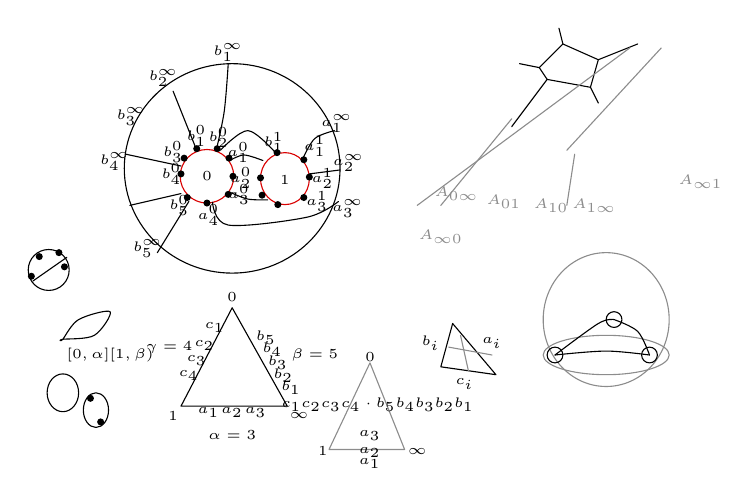
\begin{tikzpicture}[x=1mm,y=1mm,line cap=round,line join=round,font=\scriptsize]
\draw (36.5,-35.3) ellipse[x radius=13.7, y radius=13.3];
\draw[Rd] (33.3,-36.3) ellipse[x radius=3.4, y radius=3.4];
\draw[Rd] (43.2,-36.6) ellipse[x radius=3.1, y radius=3.3];
\node[inner sep=1pt] at (33.3,-36.3) {\tiny $0$};
\node[inner sep=1pt] at (43.2,-36.8) {\tiny $1$};
\draw plot[smooth, tension=0.55] coordinates {(36,-22) (35.5,-28) (34.5,-32.9)};
\draw (29,-25.5) -- (32,-33);
\draw (23,-33.5) -- (30,-35);
\draw (23.5,-40) -- (30,-38.5);
\draw (27,-46) -- (31,-39.5);
\draw plot[smooth, tension=0.55] coordinates {(36.2,-34.3) (38,-33.6) (40.4,-34.3)};
\draw plot[smooth, tension=0.55] coordinates {(36.4,-38.4) (38.5,-39.2) (41,-39.3)};
\draw plot[smooth, tension=0.55] coordinates {(34,-39.6) (36,-42.5) (46,-41.5) (50,-39.5)};
\draw plot[smooth, tension=0.55] coordinates {(45.5,-34) (47,-31.5) (49.5,-30.5)};
\draw (46.3,-36) -- (50.2,-35.5);
\draw plot[smooth, tension=0.55] coordinates {(35,-33) (38.5,-30.5) (42,-33.3)};
\node[pt] at (32,-32.8) {};
\node[pt] at (34.6,-32.8) {};
\node[pt] at (36.1,-34) {};
\node[pt] at (36.6,-36.3) {};
\node[pt] at (36,-38.6) {};
\node[pt] at (33.3,-39.7) {};
\node[pt] at (30.8,-39) {};
\node[pt] at (30,-36) {};
\node[pt] at (30.4,-34) {};
\node[pt] at (42.2,-33.3) {};
\node[pt] at (45.6,-34.2) {};
\node[pt] at (46.3,-36.4) {};
\node[pt] at (45.6,-39) {};
\node[pt] at (40.1,-36.5) {};
\node[pt] at (40.3,-38.7) {};
\node[pt] at (42.3,-39.9) {};
\node[inner sep=1pt] at (36,-20.6) {\tiny $b^\infty_1$};
\node[inner sep=1pt] at (27.8,-23.8) {\tiny $b^\infty_2$};
\node[inner sep=1pt] at (23.7,-28.7) {\tiny $b^\infty_3$};
\node[inner sep=1pt] at (21.6,-34.4) {\tiny $b^\infty_4$};
\node[inner sep=1pt] at (25.8,-45.5) {\tiny $b^\infty_5$};
\node[inner sep=1pt] at (49.8,-29.6) {\tiny $a^\infty_1$};
\node[inner sep=1pt] at (51.3,-34.6) {\tiny $a^\infty_2$};
\node[inner sep=1pt] at (51.2,-40.4) {\tiny $a^\infty_3$};
\node[inner sep=1pt] at (41.8,-32) {\tiny $b^1_1$};
\node[inner sep=1pt] at (47,-32.5) {\tiny $a^1_1$};
\node[inner sep=1pt] at (48,-36.6) {\tiny $a^1_2$};
\node[inner sep=1pt] at (47.3,-39.5) {\tiny $a^1_3$};
\node[inner sep=1pt] at (32,-31.2) {\tiny $b^0_1$};
\node[inner sep=1pt] at (34.8,-31.4) {\tiny $b^0_2$};
\node[inner sep=1pt] at (37.3,-33.3) {\tiny $a^0_1$};
\node[inner sep=1pt] at (37.6,-36.5) {\tiny $a^0_2$};
\node[inner sep=1pt] at (37.4,-38.6) {\tiny $a^0_3$};
\node[inner sep=1pt] at (33.5,-41.2) {\tiny $a^0_4$};
\node[inner sep=1pt] at (29.8,-40) {\tiny $b^0_5$};
\node[inner sep=1pt] at (28.8,-36) {\tiny $b^0_4$};
\node[inner sep=1pt] at (29,-33.2) {\tiny $b^0_3$};
\draw[-{Stealth[length=2mm]}] (13.2,-48.2) ellipse[x radius=2.6, y radius=2.6];
\draw (11.2,-49.6) -- (15.5,-46.6);
\node[pt] at (12,-46.5) {};
\node[pt] at (14.5,-46) {};
\node[pt] at (11,-49) {};
\node[pt] at (15.2,-47.8) {};
\draw[-{Stealth[length=2mm]}] plot[smooth cycle, tension=0.55] coordinates {(15,-57) (17,-54.5) (21,-53.5) (19,-56.5) (15,-57)};
\node[inner sep=1pt] at (21,-59) {\tiny $[0,\alpha][1,\beta)$};
\draw[-{Stealth[length=2mm]}] (15,-63.8) ellipse[x radius=2, y radius=2.4];
\draw (19.2,-66) ellipse[x radius=1.6, y radius=2.2];
\node[pt] at (18.5,-64.5) {};
\node[pt] at (19.8,-67.5) {};
\draw (36.5,-53) -- (30,-65.5) -- (43.5,-65.5) -- cycle;
\node[inner sep=1pt] at (36.5,-51.6) {\tiny $0$};
\node[inner sep=1pt] at (29,-66.7) {\tiny $1$};
\node[inner sep=1pt] at (45,-66.7) {\tiny $\infty$};
\node[inner sep=1pt] at (34.3,-55.5) {\tiny $c_1$};
\node[inner sep=1pt] at (33,-57.8) {\tiny $c_2$};
\node[inner sep=1pt] at (32,-59.7) {\tiny $c_3$};
\node[inner sep=1pt] at (31,-61.6) {\tiny $c_4$};
\node[inner sep=1pt] at (40.8,-56.8) {\tiny $b_5$};
\node[inner sep=1pt] at (41.6,-58.3) {\tiny $b_4$};
\node[inner sep=1pt] at (42.3,-60) {\tiny $b_3$};
\node[inner sep=1pt] at (43,-61.6) {\tiny $b_2$};
\node[inner sep=1pt] at (44,-63.2) {\tiny $b_1$};
\node[inner sep=1pt] at (33.5,-66.3) {\tiny $a_1$};
\node[inner sep=1pt] at (36.5,-66.3) {\tiny $a_2$};
\node[inner sep=1pt] at (39.5,-66.3) {\tiny $a_3$};
\node[inner sep=1pt] at (28.5,-58) {\tiny $\gamma=4$};
\node[inner sep=1pt] at (47,-59) {\tiny $\beta=5$};
\node[inner sep=1pt] at (36.5,-69.2) {\tiny $\alpha=3$};
\draw[pencil] (54,-60) -- (48.8,-71) -- (58.4,-71) -- cycle;
\node[inner sep=1pt] at (54,-59.2) {\tiny $0$};
\node[inner sep=1pt] at (48,-71.2) {\tiny $1$};
\node[inner sep=1pt] at (60,-71.2) {\tiny $\infty$};
\node[inner sep=1pt] at (55,-65.3) {\tiny $c_1c_2c_3c_4\cdot b_5b_4b_3b_2b_1$};
\node[inner sep=1pt] at (54,-69.2) {\tiny $a_3$};
\node[inner sep=1pt] at (54,-71.4) {\tiny $a_2$};
\node[inner sep=1pt] at (54,-72.8) {\tiny $a_1$};
\draw (64.5,-55) -- (63,-60.5) -- (70,-61.5) -- cycle;
\draw[pencil] (64,-58) -- (69.5,-59);
\draw[pencil] (65.5,-56.5) -- (66.5,-61);
\node[inner sep=1pt] at (61.7,-57.5) {\tiny $b_i$};
\node[inner sep=1pt] at (69.5,-57.5) {\tiny $a_i$};
\node[inner sep=1pt] at (66,-62.7) {\tiny $c_i$};
\draw (75.5,-22.5) -- (78.5,-19.5) -- (83,-21.5) -- (82,-25) -- (76.5,-24) -- cycle;
\draw (78.5,-19.5) -- (78,-17.5);
\draw (83,-21.5) -- (88,-19.5);
\draw (82,-25) -- (83,-27);
\draw (76.5,-24) -- (72,-30);
\draw (75.5,-22.5) -- (73,-22);
\draw[pencil] (60,-40) -- (87,-20);
\draw[pencil] (79,-33) -- (91,-20);
\draw[pencil] (80,-33.5) -- (79,-40);
\draw[pencil] (72,-29) -- (63,-40);
\node[inner sep=1pt,pencil] at (65,-38.5) {\tiny $A_{0\infty}$};
\node[inner sep=1pt,pencil] at (71,-39.5) {\tiny $A_{01}$};
\node[inner sep=1pt,pencil] at (77,-40) {\tiny $A_{10}$};
\node[inner sep=1pt,pencil] at (82.5,-40) {\tiny $A_{1\infty}$};
\node[inner sep=1pt,pencil] at (63,-44) {\tiny $A_{\infty 0}$};
\node[inner sep=1pt,pencil] at (96,-37) {\tiny $A_{\infty 1}$};
\draw[pencil] (84,-54.5) ellipse[x radius=8, y radius=8.5];
\draw[pencil] (84,-59) ellipse[x radius=8, y radius=2.5];
\draw (85,-54.5) circle[radius=1];
\draw (77.5,-59) circle[radius=1];
\draw (89.5,-59) circle[radius=1];
\draw plot[smooth, tension=0.55] coordinates {(77.5,-59) (83,-55) (85,-54.5)};
\draw plot[smooth, tension=0.55] coordinates {(77.5,-59) (84,-58.5) (89.5,-59)};
\draw plot[smooth, tension=0.55] coordinates {(85,-54.5) (88,-56) (89.5,-59)};
\end{tikzpicture}
\end{document}
